\documentclass[12pt,letterpaper,noanswers]{exam}
\usepackage[usenames,dvipsnames,svgnames,table]{xcolor}
\usepackage[margin=0.9in]{geometry}
\renewcommand{\familydefault}{\sfdefault}
\usepackage{multicol}
\usepackage{wrapfig}
\pagestyle{head}
\definecolor{c03}{HTML}{FFDDDD}
\header{AM 22b Class 14}{}{Mar 3: spherical}
\runningheadrule
\headrule
\usepackage{graphicx} % more modern
\usepackage{amsmath} 
\usepackage{amssymb} 
\usepackage{hyperref}
\usepackage{tcolorbox}

\usepackage[numbered,autolinebreaks,useliterate]{mcode}

\newcommand{\mb}[1]{\underline{#1}}

\begin{document}
 \pdfpageheight 11in 
  \pdfpagewidth 8.5in




% I need to review the torus trajectories...

\begin{itemize}
% \item There is a pre-class assignment (20 minutes of videos + a few WeBWorK exercises) due at 10am this Monday.  It is available on Canvas.
\itemsep0em
    % \item PSet 02 is due on Friday Feb 14th at 10am.
   % \item There is a pre-class assignment due Monday by 10am (pre-class 03).
    \item Problem set 04 is due on Thursday Mar 4th at 6pm ET.
    \item Quiz 02 will be released on Friday, and is due by Sunday at 6pm ET.
    \item There are OH on Thursday from 2-3pm this week.  The link is on the OH page in Canvas.
    \item The skill checks for C13, C14, C15 will happen on Monday Mar 8th.
\end{itemize}

\hrule
\vspace{0.2cm}

% partial derivatives, gradient
% local linearity, differential, directional deriv
% 2nd order partials + equations with partials

\noindent\textbf{Big picture}

This week we are studying integration for functions of multiple variables.  Today our focus is on spherical coordinates and triple integral practice.

\vspace{0.2cm}
\hrule
\vspace{0.2cm}

\noindent\textbf{Teams}
You will work with this team on the in-class problems today.  Share something you did on Monday instead of class.
\begin{multicols}{2}
1.  students here

\end{multicols}

%\vspace{0.2cm}
\hrule
\vspace{0.2cm}


\noindent\textbf{Skill Check C14 Practice}

\begin{questions}
\item (spherical coordinates) Sketch the region in $rz$-space associated with the region of integration in the integral below and describe the shape of the region.
\[\int_0^{2\pi}\int_0^{\pi/4}\int_0^{\frac{1}{\sqrt{2}\cos\phi}} \rho^3\sin\phi\cos\phi\ d\rho\ d\phi\ d\theta.\]
\end{questions}

\vspace{0.2cm}
\hrule
\vspace{0.2cm}

\noindent\textbf{Skill Check C14 Solution}

The shape in $rz$-space is set by the $\rho$ and $\phi$ coordinates.  $\theta$ then rotates the shape we find about the $z$-axis.  Translating from spherical to cylindrical will allow us to find the $rz$ shape.

We have $\rho = 0$ and $\rho = \frac{1}{\sqrt{2}\cos\phi}$ for our $\rho$ bounds, where $\rho = 0$ is the origin, and $\rho\cos\phi = \frac{1}{\sqrt{2}}$ can be rewritten in cylindrical coordinates as $z = \frac{1}{\sqrt{2}}$.

The $\rho$ limits tell us that we have lines radiating from the origin that extend until $z = \frac{1}{\sqrt{2}}$.

For $\phi$, we have $\phi = 0$ as the lower bound.  This is the positive $z$-axis.  And we have $\phi = \pi/4$ as the upper bound.  This is a $45$-degree line in the $rz$-plane.

The $\phi$ bounds tell us that the radial lines from $0$ to $z=1$ are part of our region when they are between the positive $z$-axis and the $45$-degree line.

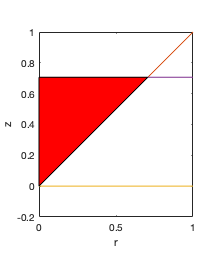
\includegraphics[scale=0.5]{img/C13skill.png}

The region is a solid cone.  (Imagine spinning this triangle around the $z$-axis through the angles $0$ to $2\pi$ to form the solid region).

\vspace{0.2cm}
\hrule
\vspace{0.2cm}

\noindent\textbf{Spherical coordinates} \S 16.5
\begin{tcolorbox}
\begin{itemize}
\itemsep0em
    \item In the \textbf{spherical coordinate} system, each point in $3$-space is represented using $0\leq \rho < \infty, 0\leq \theta\leq 2\pi, 0 \leq \phi\leq \pi.$  
    \item The spherical coordinates are most easily understood in terms of cylindrical coordinates: $z = \rho\cos\phi,$ $r = \rho\sin\phi$.
    
    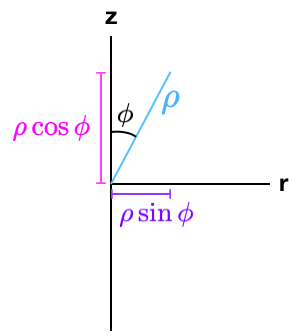
\includegraphics[width=1.7in]{img/C13spherical.png}
    
    \item Translating back to Cartesian: $x = r\cos\theta = \rho\sin\phi\cos\theta$ and $y = r\sin\theta = r\sin\phi\sin\theta$.  Note that $x^2+y^2 +z^2= \rho^2.$
    \item A region $a\leq \rho\leq b, c\leq \theta\leq d, m\leq \phi \leq n$, where all bounds are constants, will be a piece of a solid spherical ball.
    \item Why spherical?  Planets, atoms, human head, specifying robot arm (angles), 
    \end{itemize}
    \end{tcolorbox}
    
    \noindent\textbf{Example (spherical coordinates).}

The region shown in D is the region where $1\leq \rho \leq 2,$  $\pi/8\leq \theta\leq 3\pi/8,$ and $ \pi/4\leq \phi \leq 7\pi/6.$

Which of A, B, C is associated with the $\theta = c$ surfaces (for $c$ some constant)? 

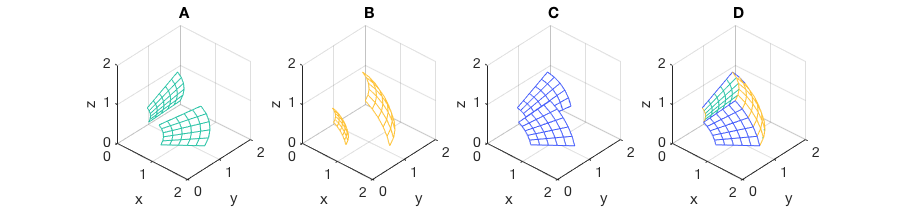
\includegraphics[width=0.9\linewidth]{img/C20p5.png}



\noindent\textbf{Example ($\phi = c$).}

In plot $A$ below are shown two surfaces on which $\phi$ is held constant.  On which surface is $\phi$ greater? 

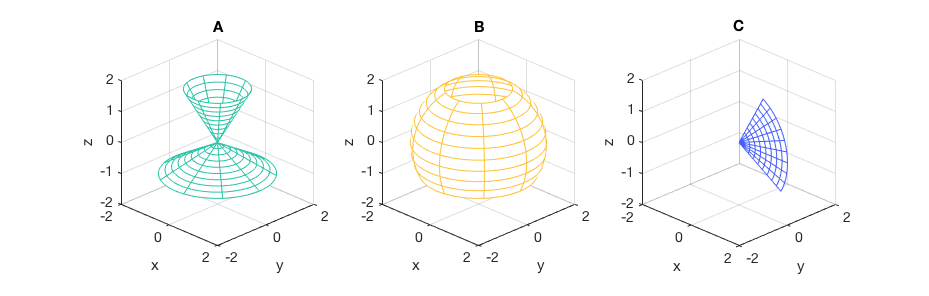
\includegraphics[width=0.7\linewidth]{img/C20p7.png}
    
    

    \noindent\textbf{Integration using spherical coordinates} \S 16.5
    \begin{tcolorbox}
    \begin{itemize}
\item The \emph{Jacobian} for the change of coordinates from Cartesian to spherical, $\displaystyle\left\vert\frac{\partial(x,y,z)}{\partial(\rho,\theta,\phi)}\right\vert$, is $\rho^2\sin\phi$ so the volume element is given by $dV = \rho^2\sin\phi\ d\overline{V} = \rho^2\sin\phi\ d\rho\ d\theta\ d\phi$.

\end{itemize} 




  %When $r$ changes by $\Delta r$, $x$ and $y$ change by approximately $\cos\theta \Delta r$ and $\sin\theta\Delta r$, respectively.  When $\theta$ changes by $\Delta \theta$, $x$ and $y$ change by approximately $-r\sin\theta\Delta\theta$ and $r\cos\theta\Delt$
\end{tcolorbox}


% \noindent\textbf{Example}

% A half-melon is approximated by the region between two spheres, one of radius $a$ and the other of radius $b$, with $0<a<b$.  Write a triple integral, including limits of integration, giving the volume of the half-melon.

% 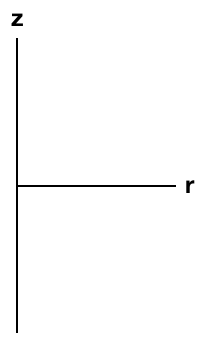
\includegraphics[height=2in]{img/C13rzaxes.png}

% \noindent\textbf{Exercises}

% Set up the following triple integrals using either cylindrical or spherical coordinates.  

% Start by sketching a cut through each region in the $rz$-half plane.
% \begin{parts}
% \item Triple integral to find the volume of the region $W$ that is inside the sphere of radius $5$ centered at the origin \textbf{and} inside the cylinder of radius $3$ centered about the $z$-axis.  \emph{This looks like a solid cylinder with spherical caps}.
% \item Triple integral to find the volume of the region $W$ inside the sphere $x^2+y^2+z^2 = 2$ and outside the double cone $z^2=x^2+y^2$ ($W$ contains the portion of the $xy$-plane within the sphere).
% %\item Redo your setups above in the other coordinate system.
% \end{parts}

% \vfill


% \eject


% \noindent\textbf{Problem}


% The figure below shows part of a spherical ball of radius $5$ cm.  Write an iterated triple integral which represents the volume of this region.

% 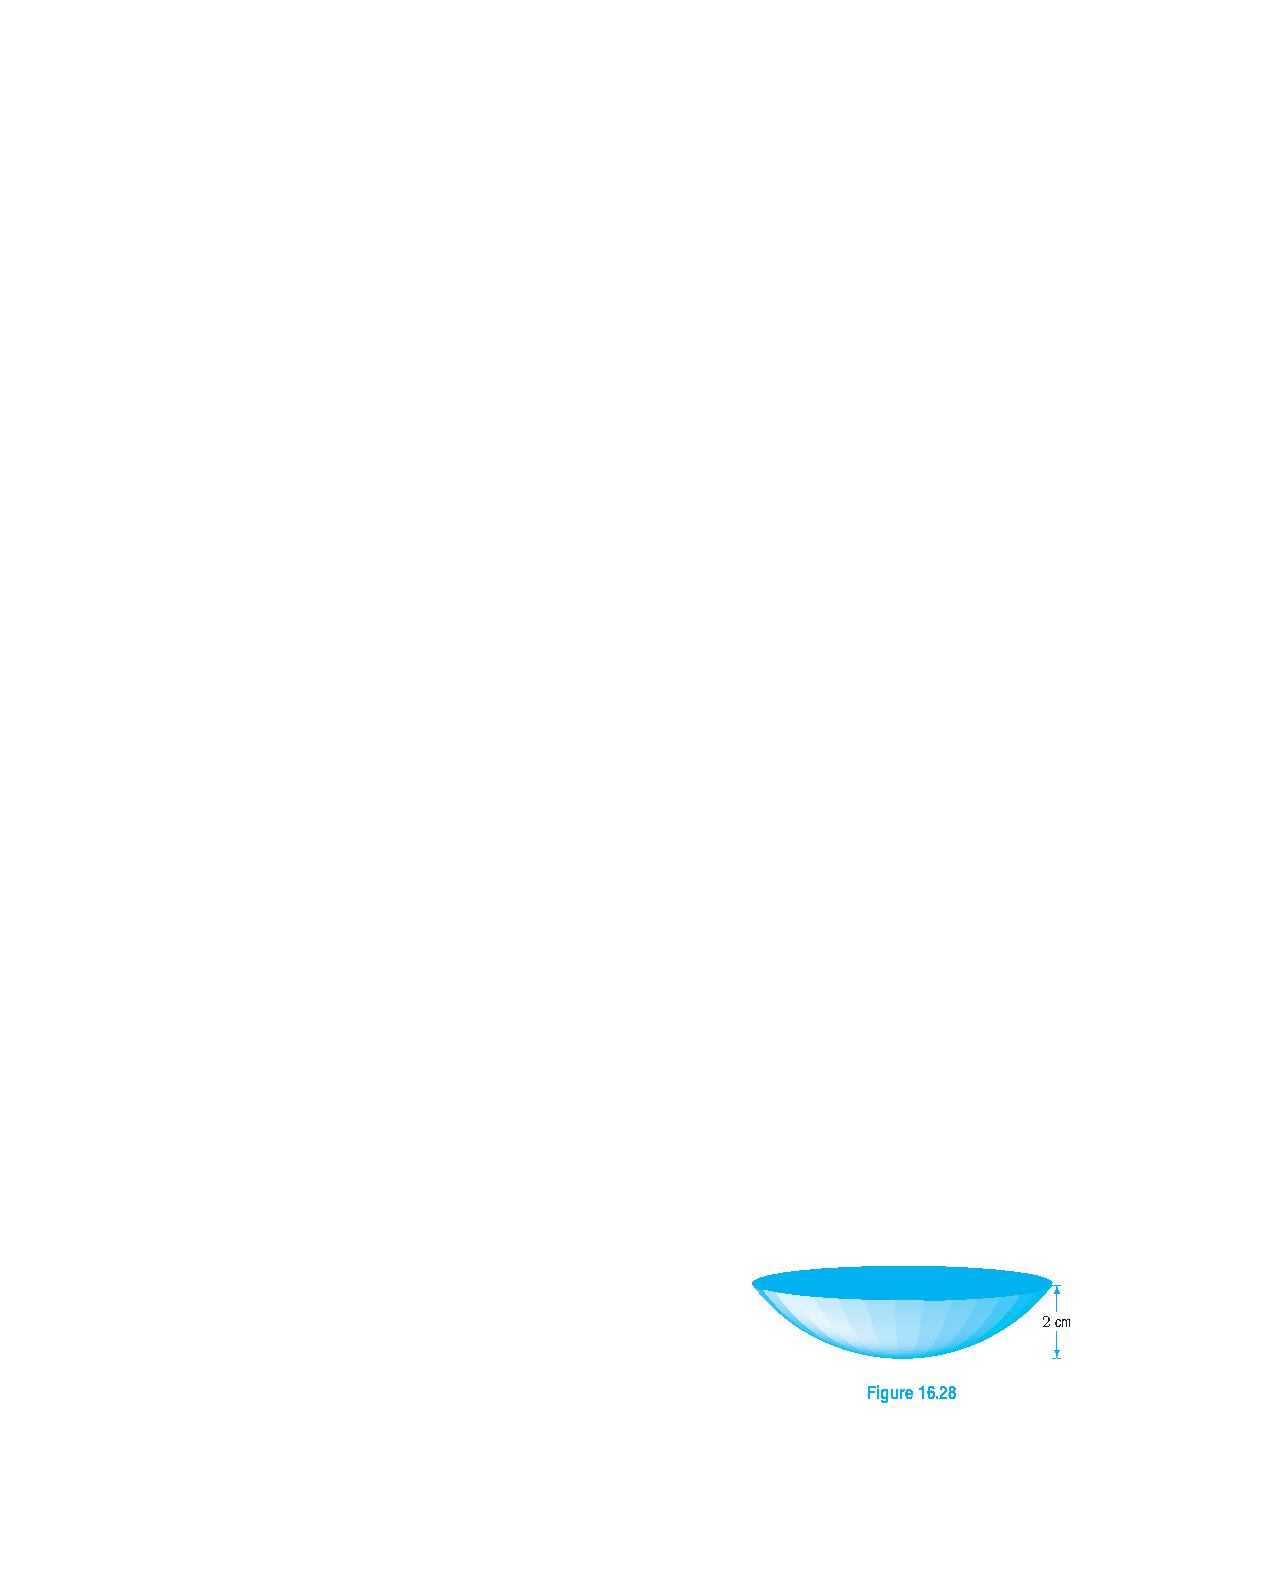
\includegraphics{img/W05p2.pdf}


% %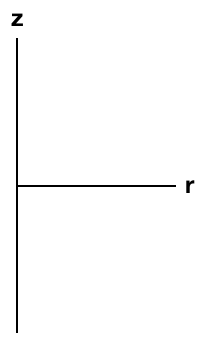
\includegraphics[height=2in]{img/C13rzaxes.png}
% \vfill

% Answers to exercises: $\int_0^{2\pi}\int_0^3\int_{-\sqrt{5-r^2}}^{\sqrt{5-r^2}}1\ r\ dz\ dr\ d\theta$.  $\int_0^{2\pi}\int_0^{\sqrt{2}}\int_{\pi/4}^{3\pi/4} \rho^2\sin\phi\ d\phi\ d\rho\ d\theta$.



\noindent\textbf{Example}

A half-melon is approximated by the region between two spheres, one of radius $a$ and the other of radius $b$, with $0<a<b$.  Write a triple integral, including limits of integration, giving the volume of the half-melon.

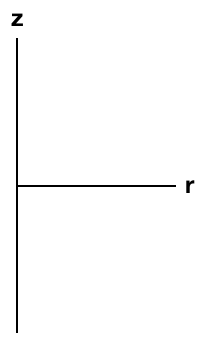
\includegraphics[height=2in]{img/C13rzaxes.png}

\noindent\textbf{Exercises}

Set up the following triple integrals using either cylindrical or spherical coordinates.  Start by sketching a cut through each region in the $rz$-half plane.
\begin{parts}
\item Triple integral to find the volume of the region $W$ that is inside the sphere of radius $5$ centered at the origin \textbf{and} inside the cylinder of radius $3$ centered about the $z$-axis.  \emph{This looks like a solid cylinder with spherical caps}.

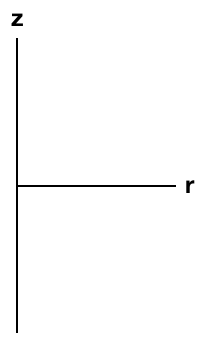
\includegraphics[height=2in]{img/C13rzaxes.png}

\item Triple integral to find the volume of the region $W$ inside the sphere $x^2+y^2+z^2 = 2$ and outside the double cone $z^2=x^2+y^2$ ($W$ contains the portion of the $xy$-plane within the sphere).

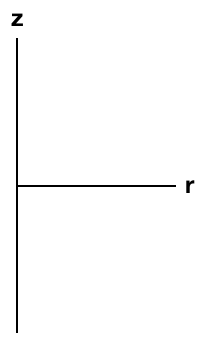
\includegraphics[height=2in]{img/C13rzaxes.png}

%\item Redo your setups above in the other coordinate system.
\end{parts}

\vfill





\noindent\textbf{Problem}


The figure below shows part of a spherical ball of radius $5$ cm.  Write an iterated triple integral which represents the volume of this region.

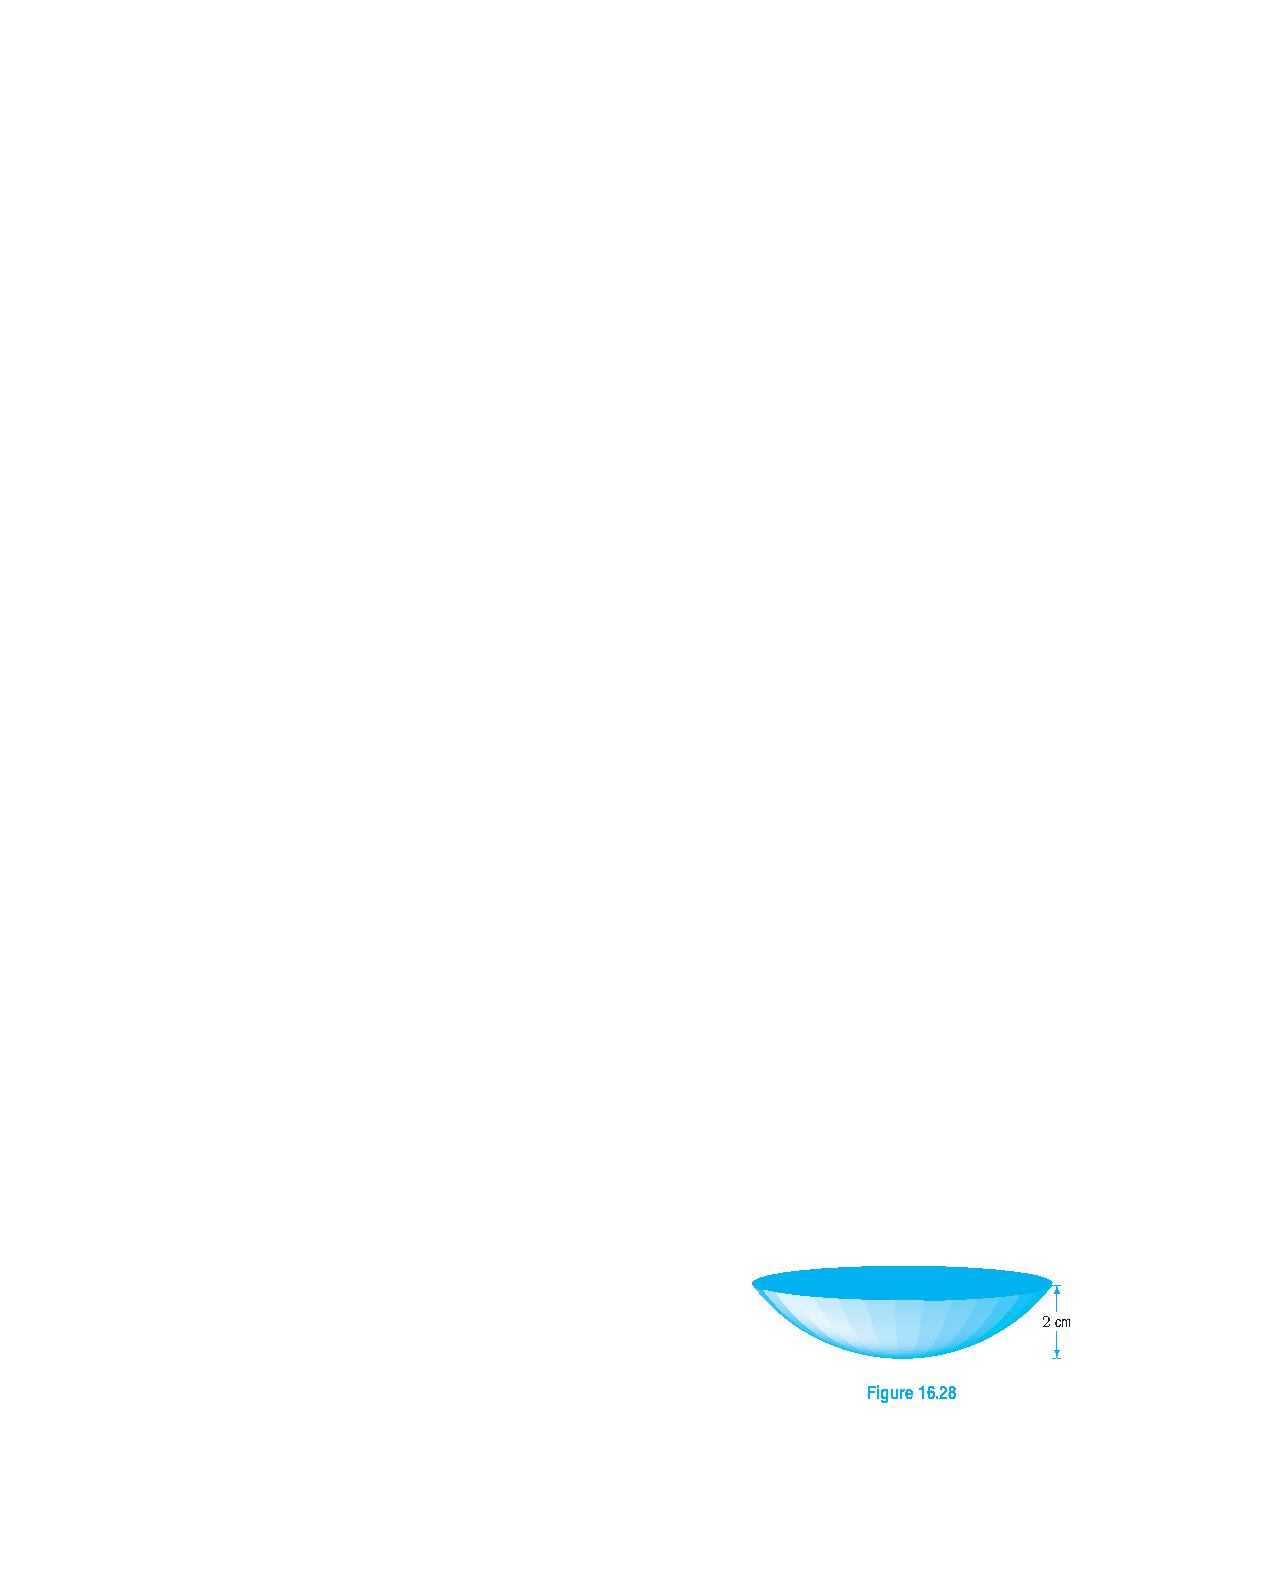
\includegraphics{img/W05p2.pdf}


%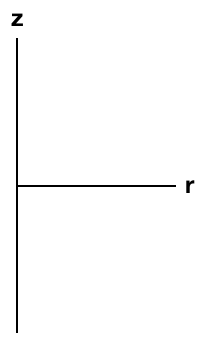
\includegraphics[height=2in]{img/C13rzaxes.png}


\noindent\textbf{Spherical integral}.  Consider the integral \[\int_0^{2\pi}\int_0^{\pi/4}\int_0^{3/\cos\phi}\rho^3\cos\phi\sin\phi\ d\rho\ d\phi\ d\theta.\]  

Identify the function of integration. Translate the integral into Cartesian coordinates.


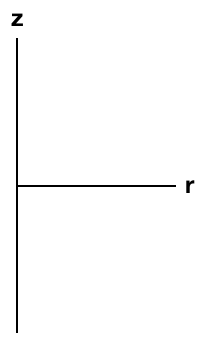
\includegraphics[height=2in]{img/C13rzaxes.png}

Answers to exercises: $\int_0^{2\pi}\int_0^3\int_{-\sqrt{5-r^2}}^{\sqrt{5-r^2}}1\ r\ dz\ dr\ d\theta$.  $\int_0^{2\pi}\int_0^{\sqrt{2}}\int_{\pi/4}^{3\pi/4} \rho^2\sin\phi\ d\phi\ d\rho\ d\theta$.

\vspace{0.2cm}
\hrule
\vspace{0.2cm}

\eject

\noindent\textbf{Probability for functions of a single variable.}
\begin{tcolorbox}
\begin{itemize}
\itemsep0em
    \item The function $p(x)$ is a \textbf{probability density function}, or pdf, if the fraction of the population for which $a\leq x\leq b$ $\displaystyle= \int_a^b p(x)\ dx$ with $\displaystyle\int_{-\infty}^{\infty}p(x)\ dx = 1$ and $p(x)\geq 0$ for all $x$.
    \item What does $\displaystyle\int_{-\infty}^{\infty}p(x)\ dx = 1$ mean in words?  This says that between $-\infty$ and $\infty$ you'll find the entire population.
    \item Why is $p(x)\geq 0$ for all $x$?  There is no interval where there would be a negative fraction of the population.
    \item $\displaystyle P(t) = \int_{-\infty}^t p(x)\ dx$ is the \textbf{cumulative distribution function.}. It gives the fraction of the population that has a value of $x$ below $t$.  $P$ is a nondecreasing function.  $\lim\limits_{t\rightarrow\infty} P(t) = 1$ and $\lim\limits_{t\rightarrow -\infty} P(t) = 0$.
    \item The fraction of the population having values of $x$ between $a$ and $b$ $\displaystyle= \int_a^b p(x)\ dx = P(b)-P(a)$.
\end{itemize}
\end{tcolorbox}

%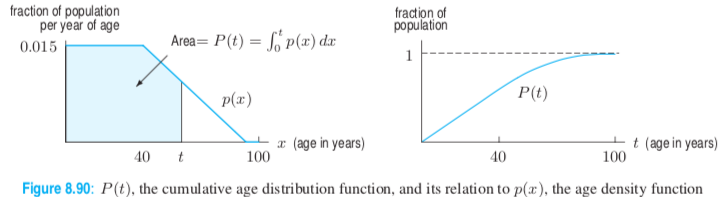
\includegraphics[width=\linewidth]{img/C20p8.png}


\noindent\textbf{Example (density and distribution functions)}. 

Match the graphs of the density functions, a,b,c, with the graphs of the distribution functions, I, II, III.  %\emph{pollQ}

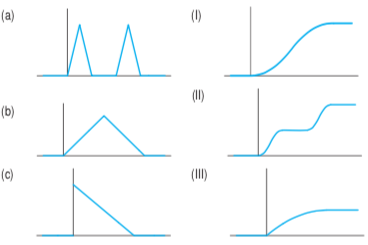
\includegraphics{img/C20p9.png}
\vfill

\eject

\noindent\textbf{Example: height of baseball players}

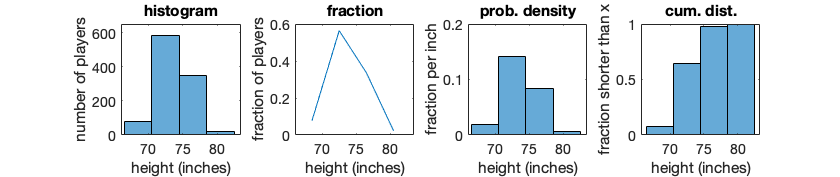
\includegraphics[width=\textwidth]{img/C14histbox4.png}

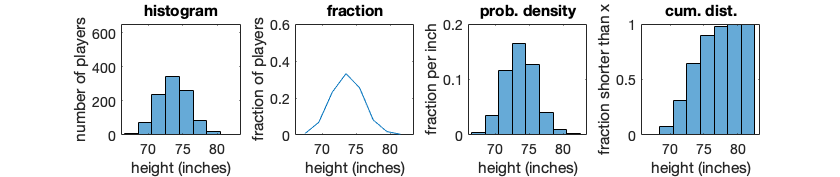
\includegraphics[width=\textwidth]{img/C14histbox2.png}

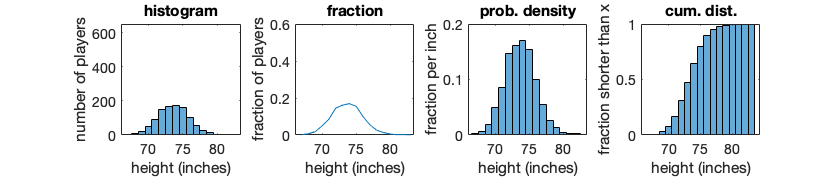
\includegraphics[width=\textwidth]{img/C14histbox1.png}


\begin{enumerate}
    \item Look at the first column (on the left).  What is changing between the different histograms? % Why is the number of players decreasing as you move down the rows?
    \item What about in the second column?
    \item What about in the third column?
    \item The shape of the plot is the same in the first column and in the third.  How would you convert from the values in the first to the values in the third?
    \item In the weight data on the next page, why does the histogram become "spiky" in the bottom row?
\end{enumerate}

\eject

\noindent\textbf{Example: weight of baseball players}

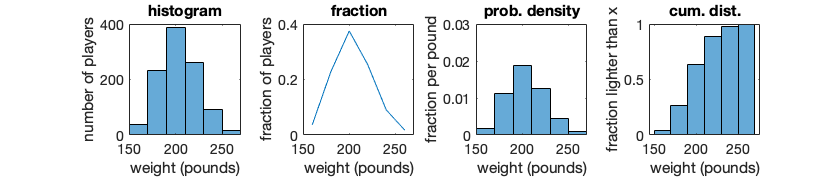
\includegraphics[width=\textwidth]{img/C14histboxweight20.png}

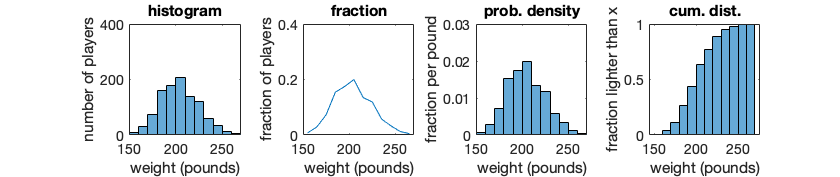
\includegraphics[width=\textwidth]{img/C14histboxweight10.png}

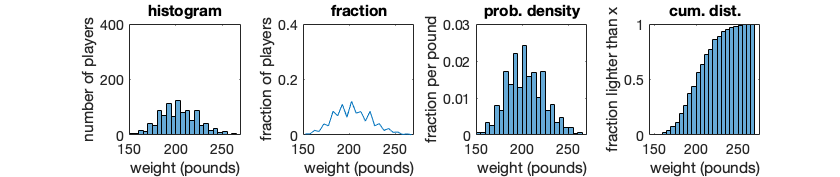
\includegraphics[width=\textwidth]{img/C14histboxweight05.png}

% \noindent\textbf{Joint probability} \S 16.6
% \begin{tcolorbox}
% \begin{itemize}
% \itemsep0em
%     \item A function $p(x,y)$ is called a \textbf{joint probability density function} or \textbf{pdf} for $x$ and $y$ if the fraction of the population that has $a\leq x\leq b$ and $c\leq y\leq d$ is given by $\int_a^b\int_c^d p(x,y)\ dy\ dx$ where $\int_{-\infty}^{\infty}\int_{-\infty}^{\infty} p(x,y)\ dy\ dx = 1$ and $p(x,y)\geq 0$ for all $x$ and $y$. 
%     \item The probability that $x$ is falling in an interval of width $\Delta x$ around $x_0$ while $y$ is falling in an interval of width $\Delta y$ about $y_0$ is approximately $p(x_0,y_0)\Delta x \Delta y.$
%   \item Two random variables are called \textbf{independent} when knowing the value of one variable does not give us any information about the distribution of the other variable.
% \end{itemize}
% \end{tcolorbox}


% \vspace{0.2cm}
% \hrule
% \vspace{0.2cm}

% \noindent\textbf{Example (joint probability distribution)}.
% The plots below are showing information about the distribution of height and weight for major league baseball players.
% The upper right graph, showing fraction per box area, is an approximation of the joint probability density function (pdf).  \\

% Based on the pdf, are height and weight independent?



% %\emph{pollQ}

% \hspace{-0.5in}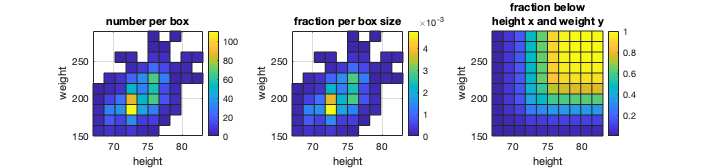
\includegraphics[width=0.9\linewidth]{img/C14joint.png}

% \emph{They are independent if at each value of weight the height has an identical probability distribution and vice versa.}

% %\vfill
% %\eject





% \noindent\textbf{Example (joint probability distribution)}.
% I generated $40000$ pairs of random numbers $(x,y)$ with $0\leq x\leq 1$ and $0\leq y \leq 1$.  Each number in the pair was drawn using a uniform distribution from the interval $[0,1]$.  I binned the numbers using $100$ boxes (a $10$ by $10$ grid).

% \begin{verbatim}
% data = rand(40000,2);
% boxes = 10;
% subplot(2,2,2)
% histogram2(dat2(:,1),dat2(:,2),boxes,'normalization','pdf','DisplayStyle','tile')
% xlabel('x'); ylabel('y'); title('fraction per box area')
% set(gca,'fontsize',14)
% caxis([0 2])
% \end{verbatim}

% An approximation for the joint probability density function (pdf) is shown on the upper right (it was make using the code given above).

% Let $p(x,y)$ be the pdf.  $p(x,y) \approx k$ where $k$ is a constant.  Find an estimate for $k$.

% %\emph{pollQ}

% 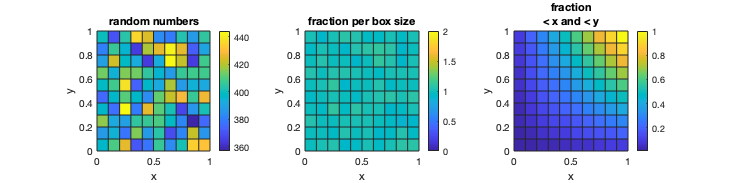
\includegraphics[width=\linewidth]{img/C14simulation.png}



% \noindent\textbf{Example (probability density)}.  A point is chosen at random from the region $R$ in the $xy$-plane containing all points $(x,y)$ such that $0\leq x\leq 2, 0\leq y\leq 2$.  ``At random'' means that the density function is constant on $R$.  

% % The density is the fraction of points per unit area.

% Which of the following is the joint probability density function?

% \begin{oneparcheckboxes}
% \choice $p(x,y) = 1/4$
% \choice $p(x,y) = 1/2$
% \choice $p(x,y) = 1$
% \choice $p(x,y) = 2$
% \end{oneparcheckboxes}



% \vfill

% \noindent\textbf{Example (probability)}.  For the joint probability density function and region $R$ above, what is the probability that we would choose a point such that $x > y$?

% Shade the region in $R$ where $x>y$ to help you think about this.

% 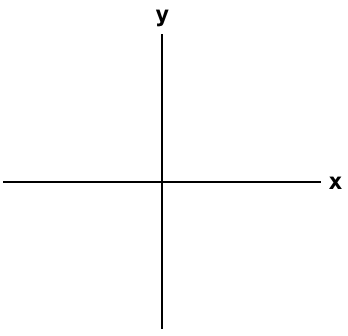
\includegraphics[height=1.5in]{img/C02axes-2.png}


% %\emph{pollQ}


\end{document}